\chapter{\texorpdfstring{Quantitative Analysis}{Quantitative Analysis}}
\label{ch:20}
\lecturemeta{Lezione 20 \quad\textbullet\quad 2026-07-04 \quad\textbullet\quad Roberto Bruni}{Dumas et al., \emph{Fundamentals of Business Process Management}, Ch.7}

Fin qui ci siamo chiesti se un processo fosse \textbf{corretto} (soundness, verification): domande qualitative come "c'è un deadlock?", "tutti i casi terminano?". Questa lezione cambia registro e affronta le domande \textbf{quantitative}: quanto è \textbf{veloce}, quanto \textbf{costa}, quanti casi si riescono a gestire in un'ora? È il campo della \textbf{performance analysis}.

\begin{boxnote}{Verification vs performance analysis}
\begin{itemize}
\item \textbf{Validation}: il modello rispecchia la realtà?
\item \textbf{Verification}: domande \emph{qualitative} — c'è un deadlock possibile? un caso specifico può sempre essere gestito con successo? due task si possono eseguire in qualsiasi ordine?
\item \textbf{Performance analysis}: domande \emph{quantitative} — quanti casi si gestiscono in un'ora? qual è il tempo medio di attraversamento? quante risorse extra servono?
\end{itemize}
\end{boxnote}

\section{\texorpdfstring{Le dimensioni della performance}{Le dimensioni della performance}}

Qualunque azienda vuole processi più \textbf{veloci}, più \textbf{economici} e \textbf{migliori}. Questi tre aggettivi corrispondono a tre dimensioni misurabili.

\begin{boxdefinition}{Le tre dimensioni}
\begin{itemize}
\item \textbf{Time} (veloce): quanto tempo richiede il processo.
\item \textbf{Finance} (economico): quanto costa eseguirlo.
\item \textbf{Quality} (migliore): quanto è soddisfacente per chi lo vive, dentro e fuori l'azienda.
\end{itemize}
\end{boxdefinition}

Per misurare una dimensione serve una quantità \emph{precisa e univoca}: un \textbf{Key Performance Indicator (KPI)}.

\subsection{\texorpdfstring{Time}{Time}}

\begin{boxdefinition}{Le tre componenti del tempo}
\begin{itemize}
\item \textbf{Cycle time}: il tempo totale per gestire un caso, dall'inizio alla fine.
\item \textbf{Processing time} (o \emph{service time}): il tempo che le risorse spendono \textbf{effettivamente} lavorando sul caso.
\item \textbf{Waiting time}: il tempo che il caso passa \textbf{in attesa} (in coda, per l'indisponibilità di una risorsa, ecc.), senza che nessuno vi lavori sopra.
\end{itemize}

Gli obiettivi tipici riguardano il cycle time: ridurne la \textbf{media}, ridurne il \textbf{massimo}, oppure rispettare un tempo \textbf{concordato} col cliente.
\end{boxdefinition}

\subsection{\texorpdfstring{Finance}{Finance}}

\begin{boxnote}{Tipi di costo}
\begin{itemize}
\item \textbf{Fixed cost}: costi fissi, indipendenti dall'intensità di lavorazione (infrastruttura, manutenzione).
\item \textbf{Variable cost}: correlati positivamente a qualche quantità (volume di vendite, nuove assunzioni).
\item \textbf{Operational cost}: legati direttamente all'\textbf{output} del processo (es. costo del lavoro per produrre un bene). È spesso il bersaglio principale del process redesign — anche se automatizzare un task, pur riducendo il costo del lavoro, introduce costi incidentali di sviluppo e manutenzione dell'applicazione.
\end{itemize}
\end{boxnote}

\subsection{\texorpdfstring{Quality}{Quality}}

\begin{boxnote}{Due prospettive}
\begin{itemize}
\item \textbf{External quality}: dal punto di vista del \textbf{cliente} (soddisfazione per il prodotto, per come è stato gestito il processo — quantità, rilevanza e tempestività delle informazioni ricevute).
\item \textbf{Internal quality}: dal punto di vista di \textbf{chi esegue} il processo (controllo sul proprio lavoro, varietà, sfide).
\end{itemize}

Spesso la external quality si misura \emph{in termini di tempo} (es. percentuale di scadenze rispettate): per questo, in pratica, una misura di qualità legata al tempo viene classificata sotto la dimensione \textbf{time}.
\end{boxnote}

\subsection{\texorpdfstring{Derivare i KPI}{Derivare i KPI}}

Un metodo pratico per passare da un obiettivo generico a un KPI misurabile:

\begin{boxnote}{Tre passi}
\begin{enumerate}
\item Formulare l'obiettivo ad \textbf{alto livello} (uno stato desiderabile);
\item per ogni obiettivo, individuare \textbf{dimensione} e \textbf{funzione di aggregazione} (count, average, variance, min, max, …) e derivarne uno o più KPI;
\item fissare un \textbf{target} per ciascun KPI.
\end{enumerate}
\end{boxnote}

\begin{boxexample}{Un ristorante che vuole migliorare il servizio}
Obiettivo: "i clienti dovrebbero essere serviti entro 30 minuti". KPI: \textbf{ST30} = percentuale di clienti serviti entro 30 minuti, target $\ge 97\%$. Oppure, più ambizioso: \textbf{ST15} (serviti entro 15 minuti, target $\ge 85\%$), o direttamente \textbf{AMDT} = tempo medio di consegna del pasto, target $\le 15'$.
\end{boxexample}

\section{\texorpdfstring{Flow analysis: dai tempi delle attività al tempo del processo}{Flow analysis: dai tempi delle attività al tempo del processo}}

La \textbf{flow analysis} è una famiglia di tecniche per stimare la performance \textbf{complessiva} di un processo a partire dalla performance \textbf{delle singole attività} — analogamente si può calcolare il costo medio del processo dal costo di ogni attività, o il tasso d'errore complessivo dai tassi d'errore locali. Qui ci concentriamo sul caso più istruttivo: il \textbf{cycle time}.

\begin{boxdefinition}{Cycle time analysis}
Il \textbf{cycle time} (CT) di un'attività o processo è la differenza fra l'istante di completamento e quello in cui il caso è pronto per essere eseguito. L'assunzione di base: sono note le \textbf{medie} dei tempi di ciascuna attività coinvolta (activity time = waiting time + processing time).
\end{boxdefinition}

Si analizzano quattro \textbf{pattern di flusso} ricorrenti, componendoli via via su strutture più complesse: \textbf{sequenza}, \textbf{cammini alternativi} (XOR), \textbf{cammini paralleli} (AND), \textbf{rework} (cicli). Notazione: $CT$ indica il cycle time medio; $CT_A, CT_B, \dots$ quello delle singole attività.

\subsection{\texorpdfstring{Sequenza}{Sequenza}}

\begin{boxtheorem}{Sequenza}
Il cycle time di un frammento puramente sequenziale è la \textbf{somma} dei cycle time delle attività: \(CT = \sum_{i=1}^n CT_i\)
\end{boxtheorem}

\begin{figure}[!htb]
\centering
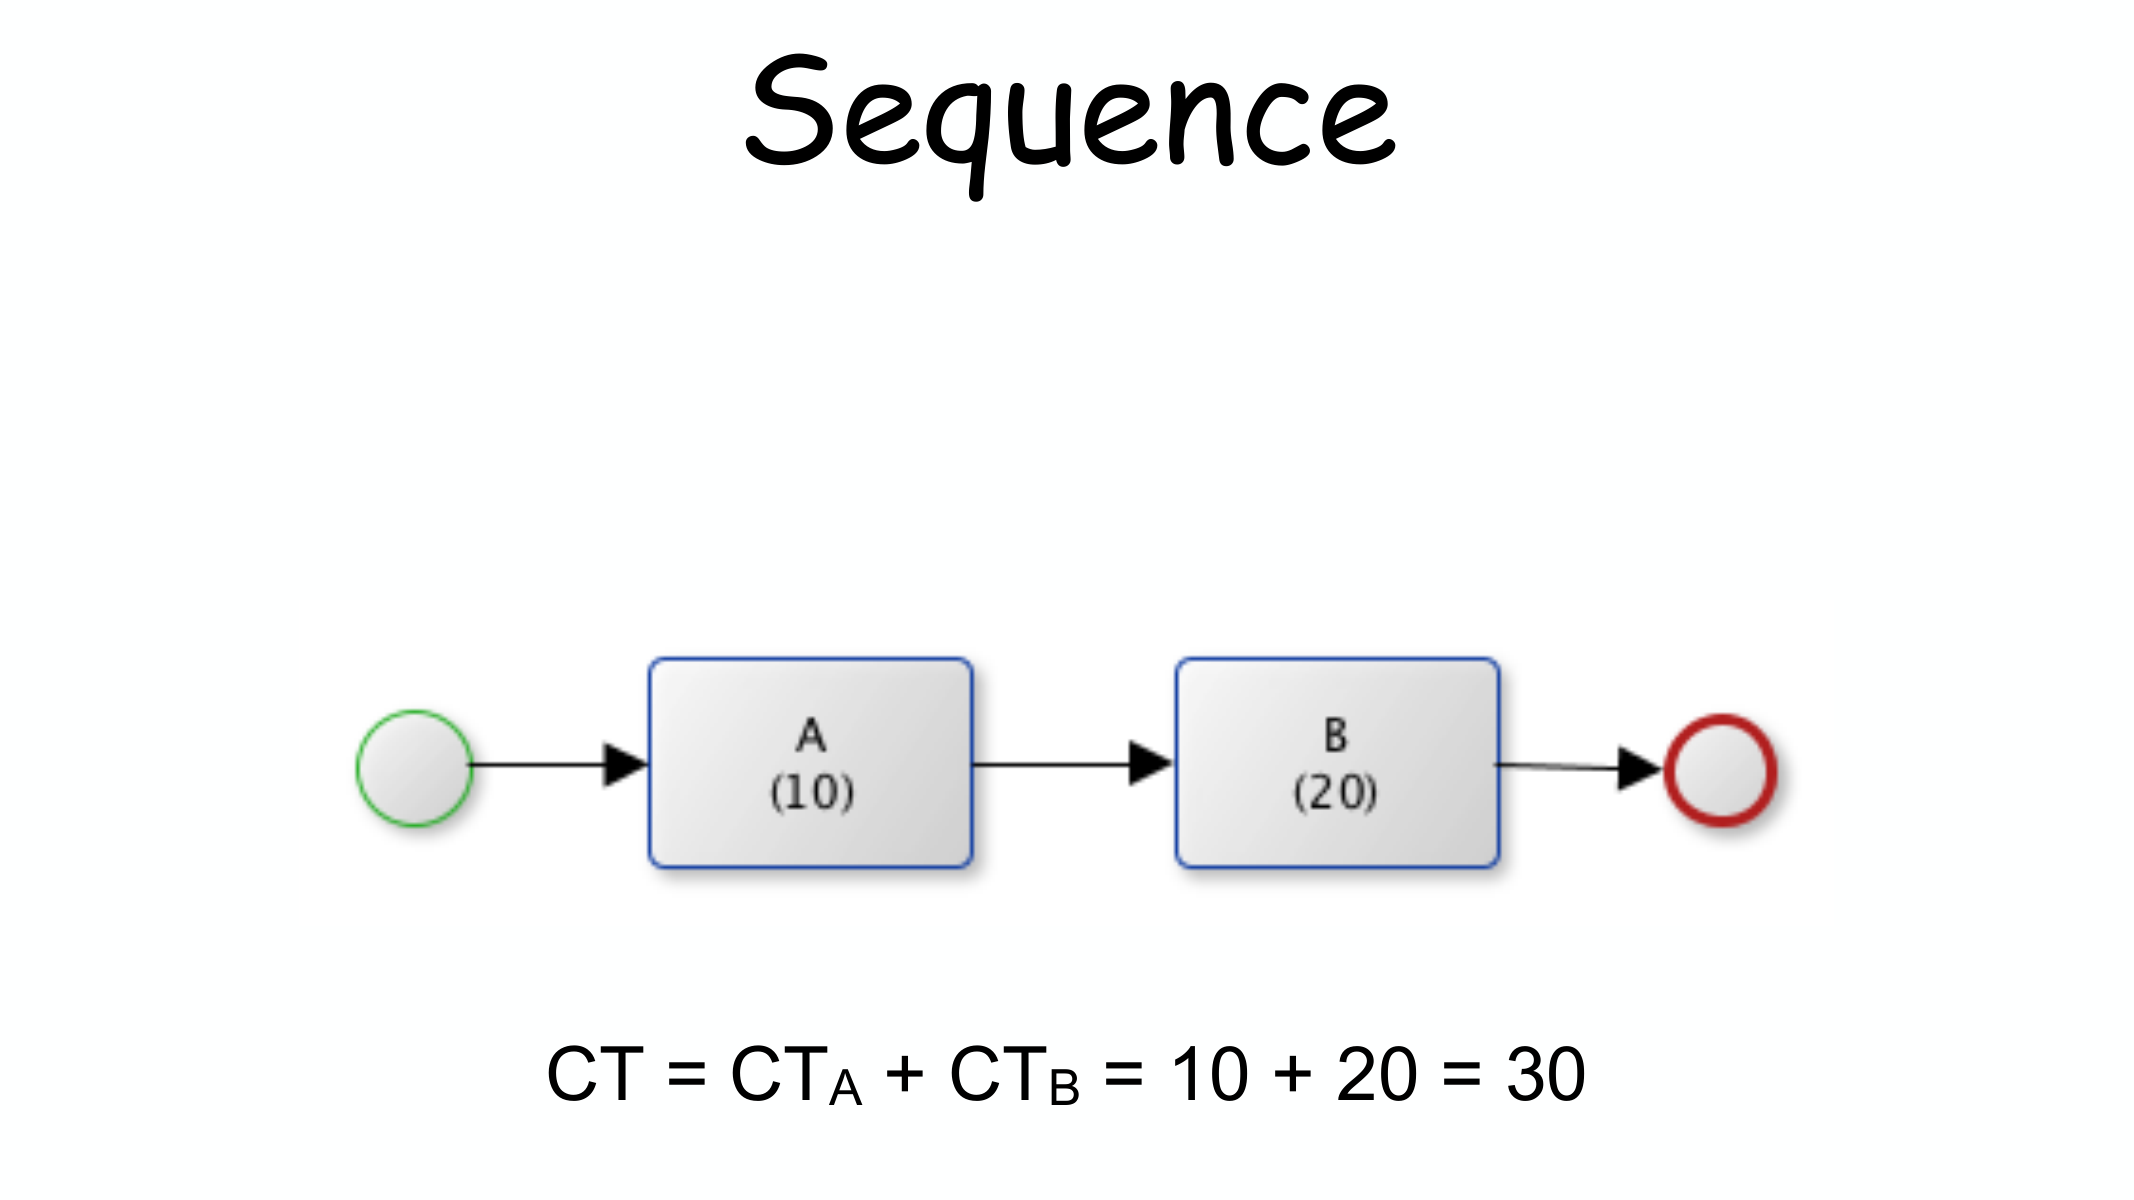
\includegraphics[width=0.74\linewidth,height=0.34\textheight,keepaspectratio]{images/20-quantitative_p30_sequence.png}
\caption{Sequenza: $CT = CT_A + CT_B = 10+20=30$. Ovvio, ma è il mattone su cui si costruiscono gli altri pattern.}
\end{figure}

\subsection{\texorpdfstring{Cammini alternativi (XOR)}{Cammini alternativi (XOR)}}

Con uno XOR-split/join il processo segue \textbf{un solo} ramo per caso, ma rami diversi in casi diversi: il cycle time medio dipende da \textbf{quanto spesso} ciascun ramo viene preso.

\begin{boxdefinition}{Branching probability}
La \textbf{branching probability} $p_i$ di un ramo è la frequenza con cui quel ramo viene scelto in un dato gateway. Vale sempre $\sum_i p_i = 1$.
\end{boxdefinition}

\begin{boxtheorem}{XOR-block}
Il cycle time di uno \textbf{XOR-block} (il frammento fra uno XOR-split e il corrispondente join) è la \textbf{media pesata} dei cycle time dei rami: \(CT = \sum_{i=1}^n p_i \cdot CT_i\)
\end{boxtheorem}

\begin{figure}[!htb]
\centering
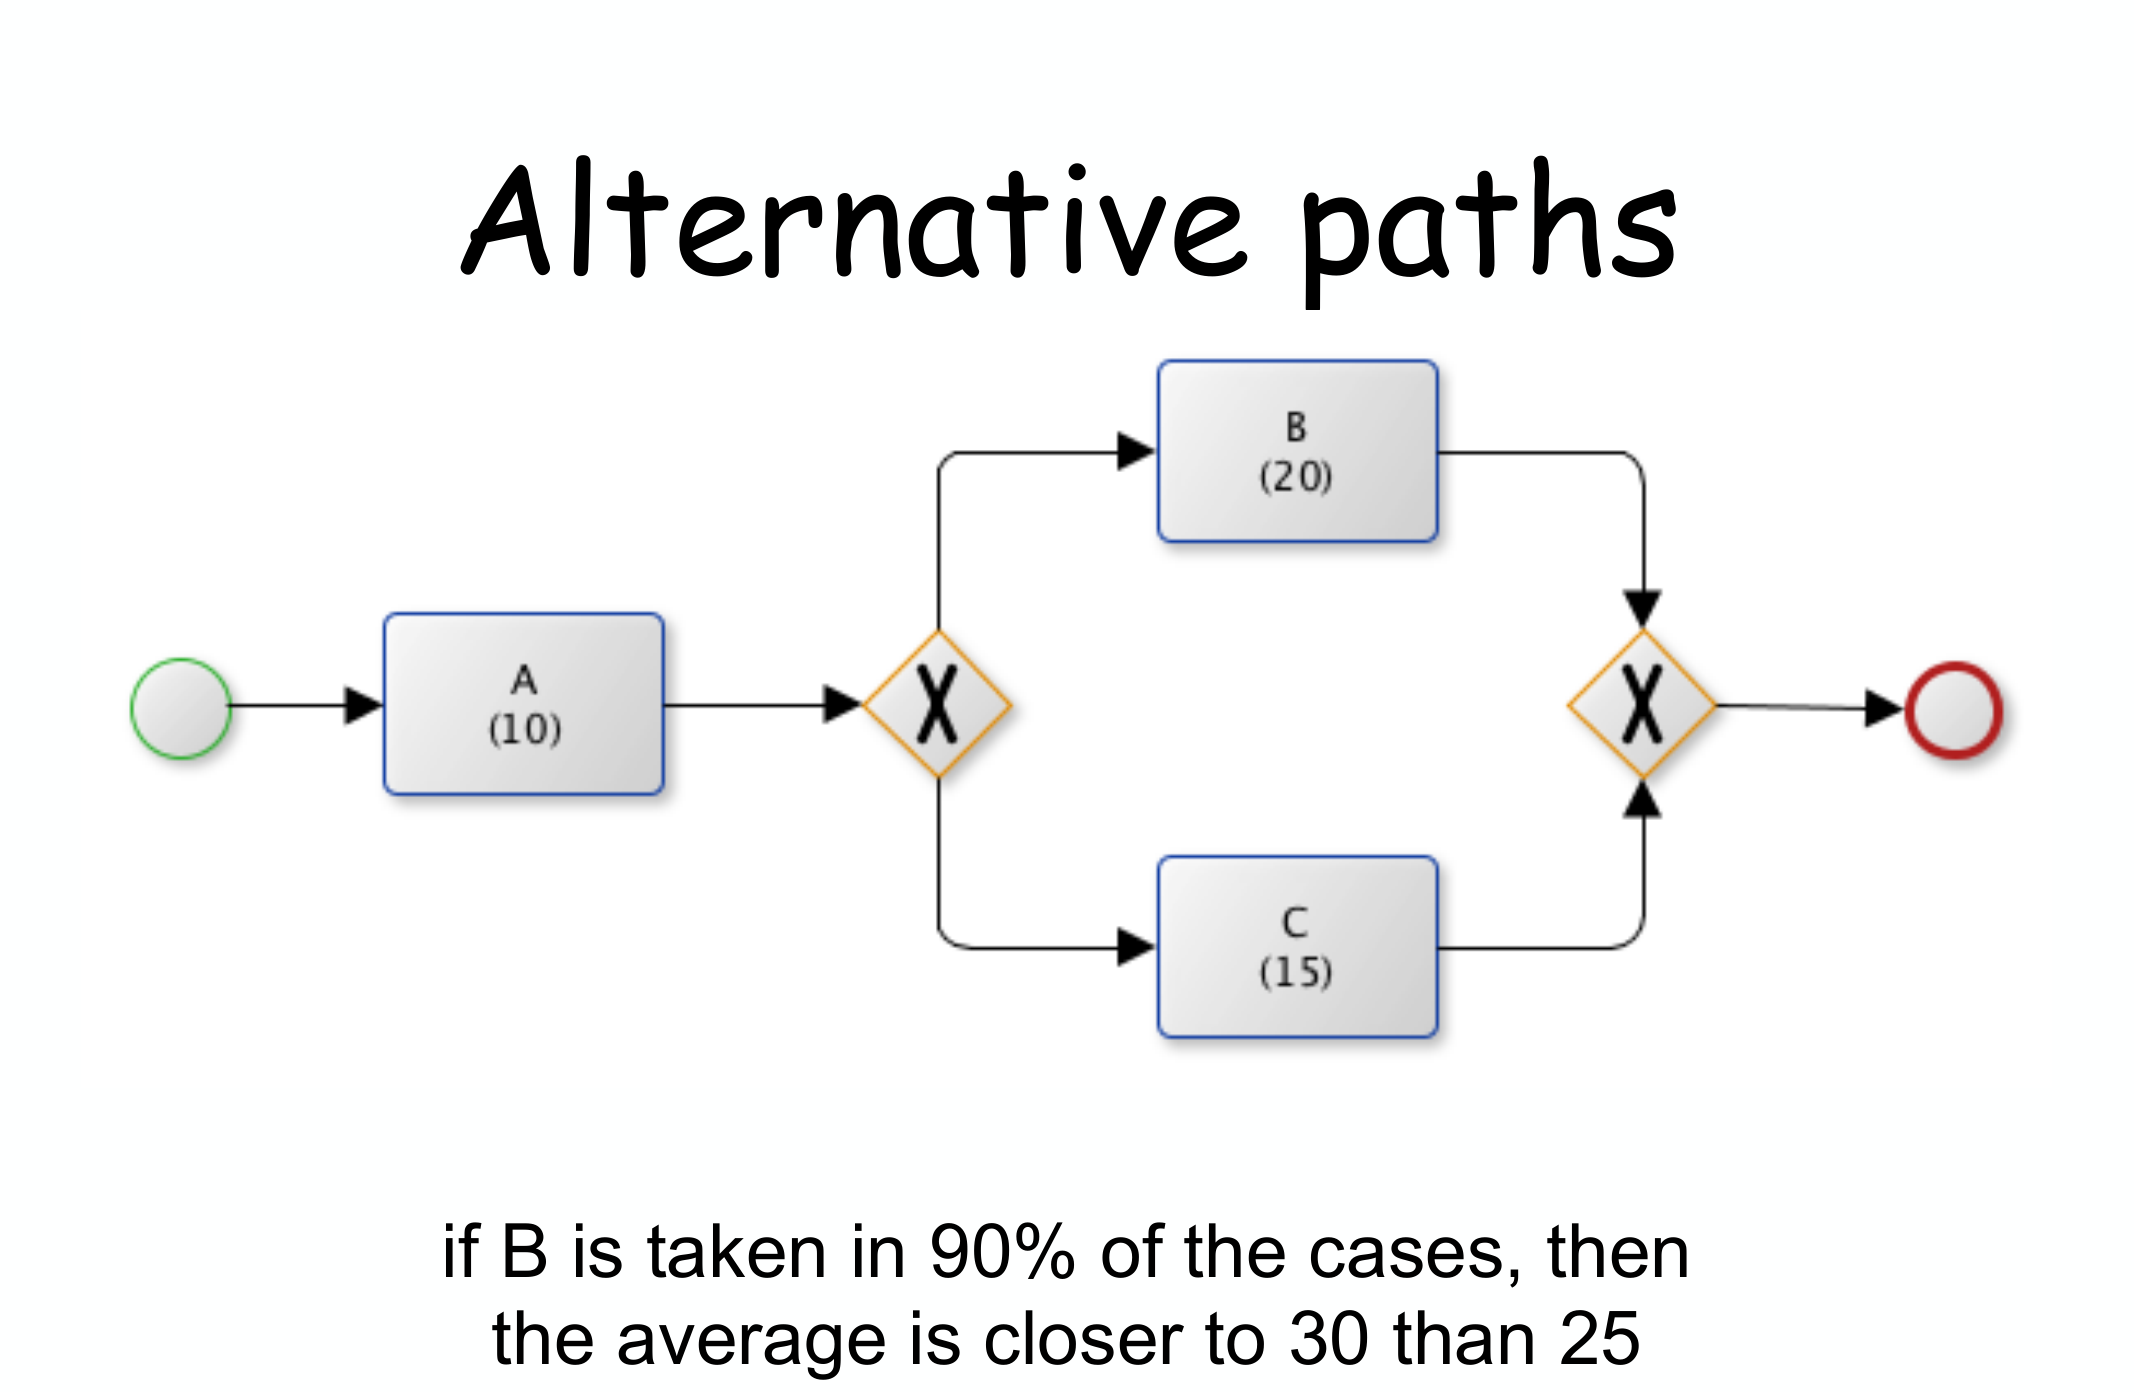
\includegraphics[width=0.74\linewidth,height=0.34\textheight,keepaspectratio]{images/20-quantitative_p35_alternative-paths.png}
\caption{Se \textbf{B} ($CT_B=20$) è preso nel 90\% dei casi e \textbf{C} ($CT_C=15$) nel 10\%, la media pesata è $0.9\cdot20+0.1\cdot15=19.5$, vicina a 30 (=$CT_A+CT_B$) proprio perché il ramo lento è quello più frequente.}
\end{figure}

\subsection{\texorpdfstring{Cammini paralleli (AND)}{Cammini paralleli (AND)}}

Con un AND-split i rami partono \textbf{insieme}; il caso prosegue solo quando \textbf{tutti} sono completati — quindi conta il ramo più lento, non la somma.

\begin{boxtheorem}{AND-block}
Il cycle time di un \textbf{AND-block} è il cycle time del ramo \textbf{più lento}: \(CT = \max_i \{CT_i\}\)
\end{boxtheorem}

\begin{figure}[!htb]
\centering
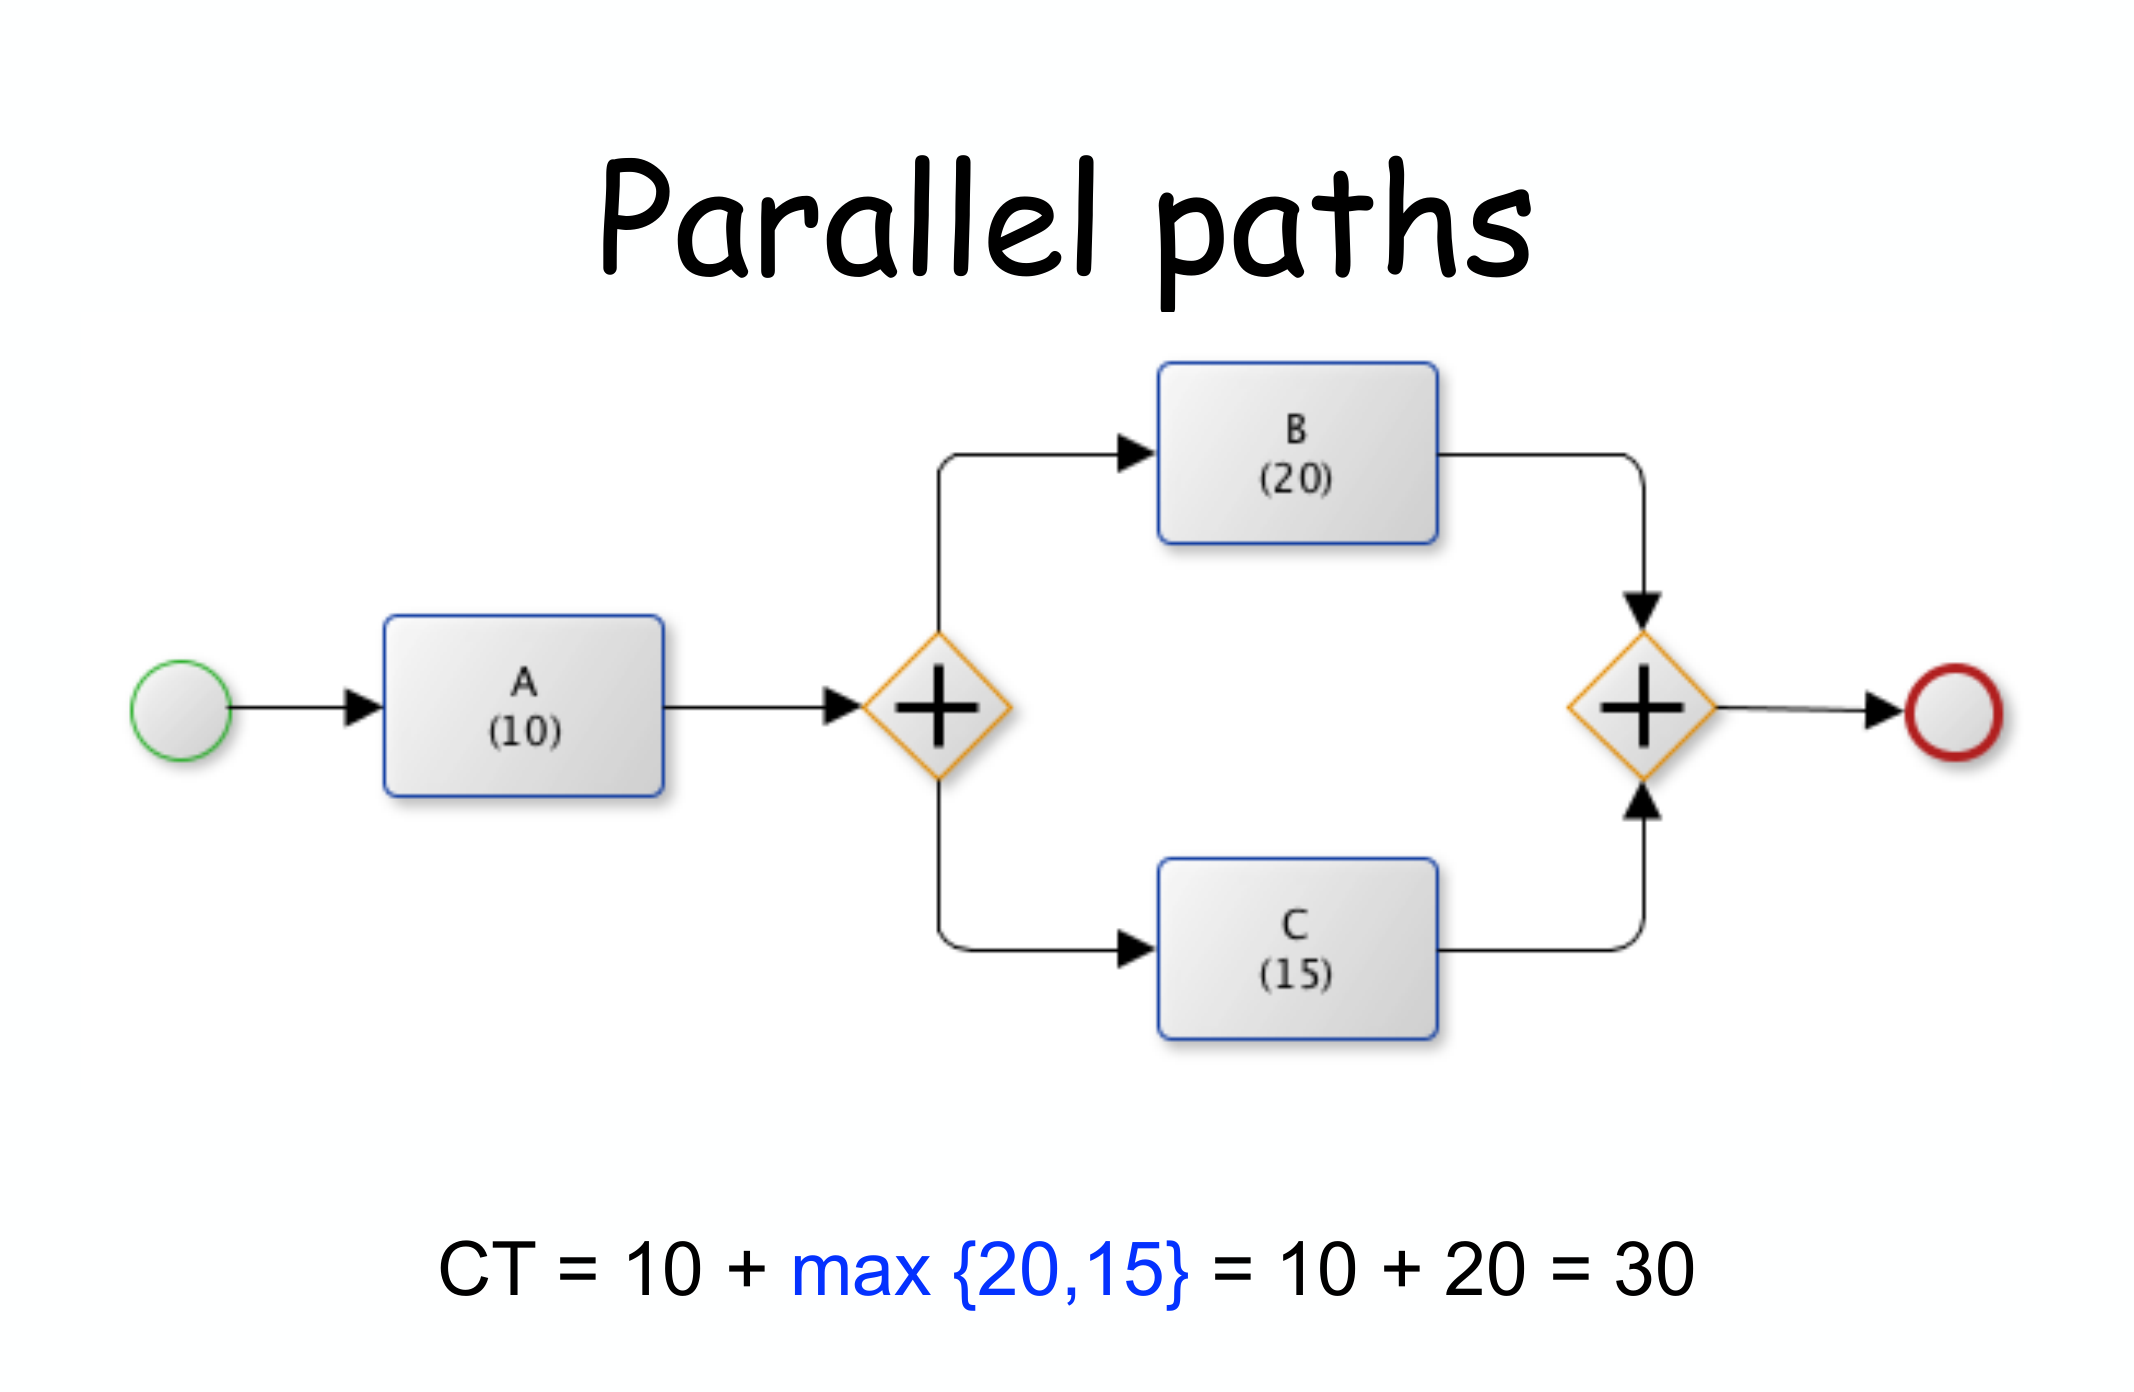
\includegraphics[width=0.74\linewidth,height=0.34\textheight,keepaspectratio]{images/20-quantitative_p41_parallel-paths.png}
\caption{$CT = CT_A + \max\{CT_B,CT_C\} = 10+\max\{20,15\}=30$: \textbf{non} $10+20+15=45$, perché B e C avvengono \textbf{contemporaneamente}, non uno dopo l'altro.}
\end{figure}

Sequenza, XOR e AND si combinano liberamente in un processo strutturato a blocchi, sommando/mediando/massimizzando via via ogni sotto-blocco.

\subsection{\texorpdfstring{Rework loop: cicli}{Rework loop: cicli}}

Il pattern più delicato è il \textbf{rework}: un frammento $P$ che può essere ripetuto, con una certa probabilità $r$ di tornare indietro invece di uscire. Ci sono due varianti, a seconda che $P$ venga eseguito \textbf{almeno una volta} oppure anche \textbf{zero volte}.

\begin{boxdefinition}{Rework probability}
La \textbf{rework probability} $r$ è la frequenza con cui, dopo aver eseguito $P$, si decide di \textbf{ripeterlo} invece di procedere (probabilità complementare $1-r$ di uscire).
\end{boxdefinition}

Il ragionamento è lo stesso della \hyperref[ch:14]{serie geometrica}: $P$ viene eseguito $1$ volta con probabilità $(1-r)$, $2$ volte con probabilità $r(1-r)$, $3$ volte con probabilità $r^2(1-r)$, e così via — sommando il contributo di ognuna di queste possibilità pesata per la sua probabilità si ottiene una serie che converge a una forma chiusa sorprendentemente semplice.

\begin{boxtheorem}{Rework loop (1 o più volte)}
Se $P$ viene eseguito \textbf{almeno una volta} (esce solo dopo il primo tentativo, con probabilità $1-r$ di fermarsi ogni volta): \(CT = \sum_{i=1}^{\infty} i \cdot CT_P \cdot r^{i-1}(1-r) = \frac{CT_P}{1-r}\)
\end{boxtheorem}

\begin{figure}[!htb]
\centering
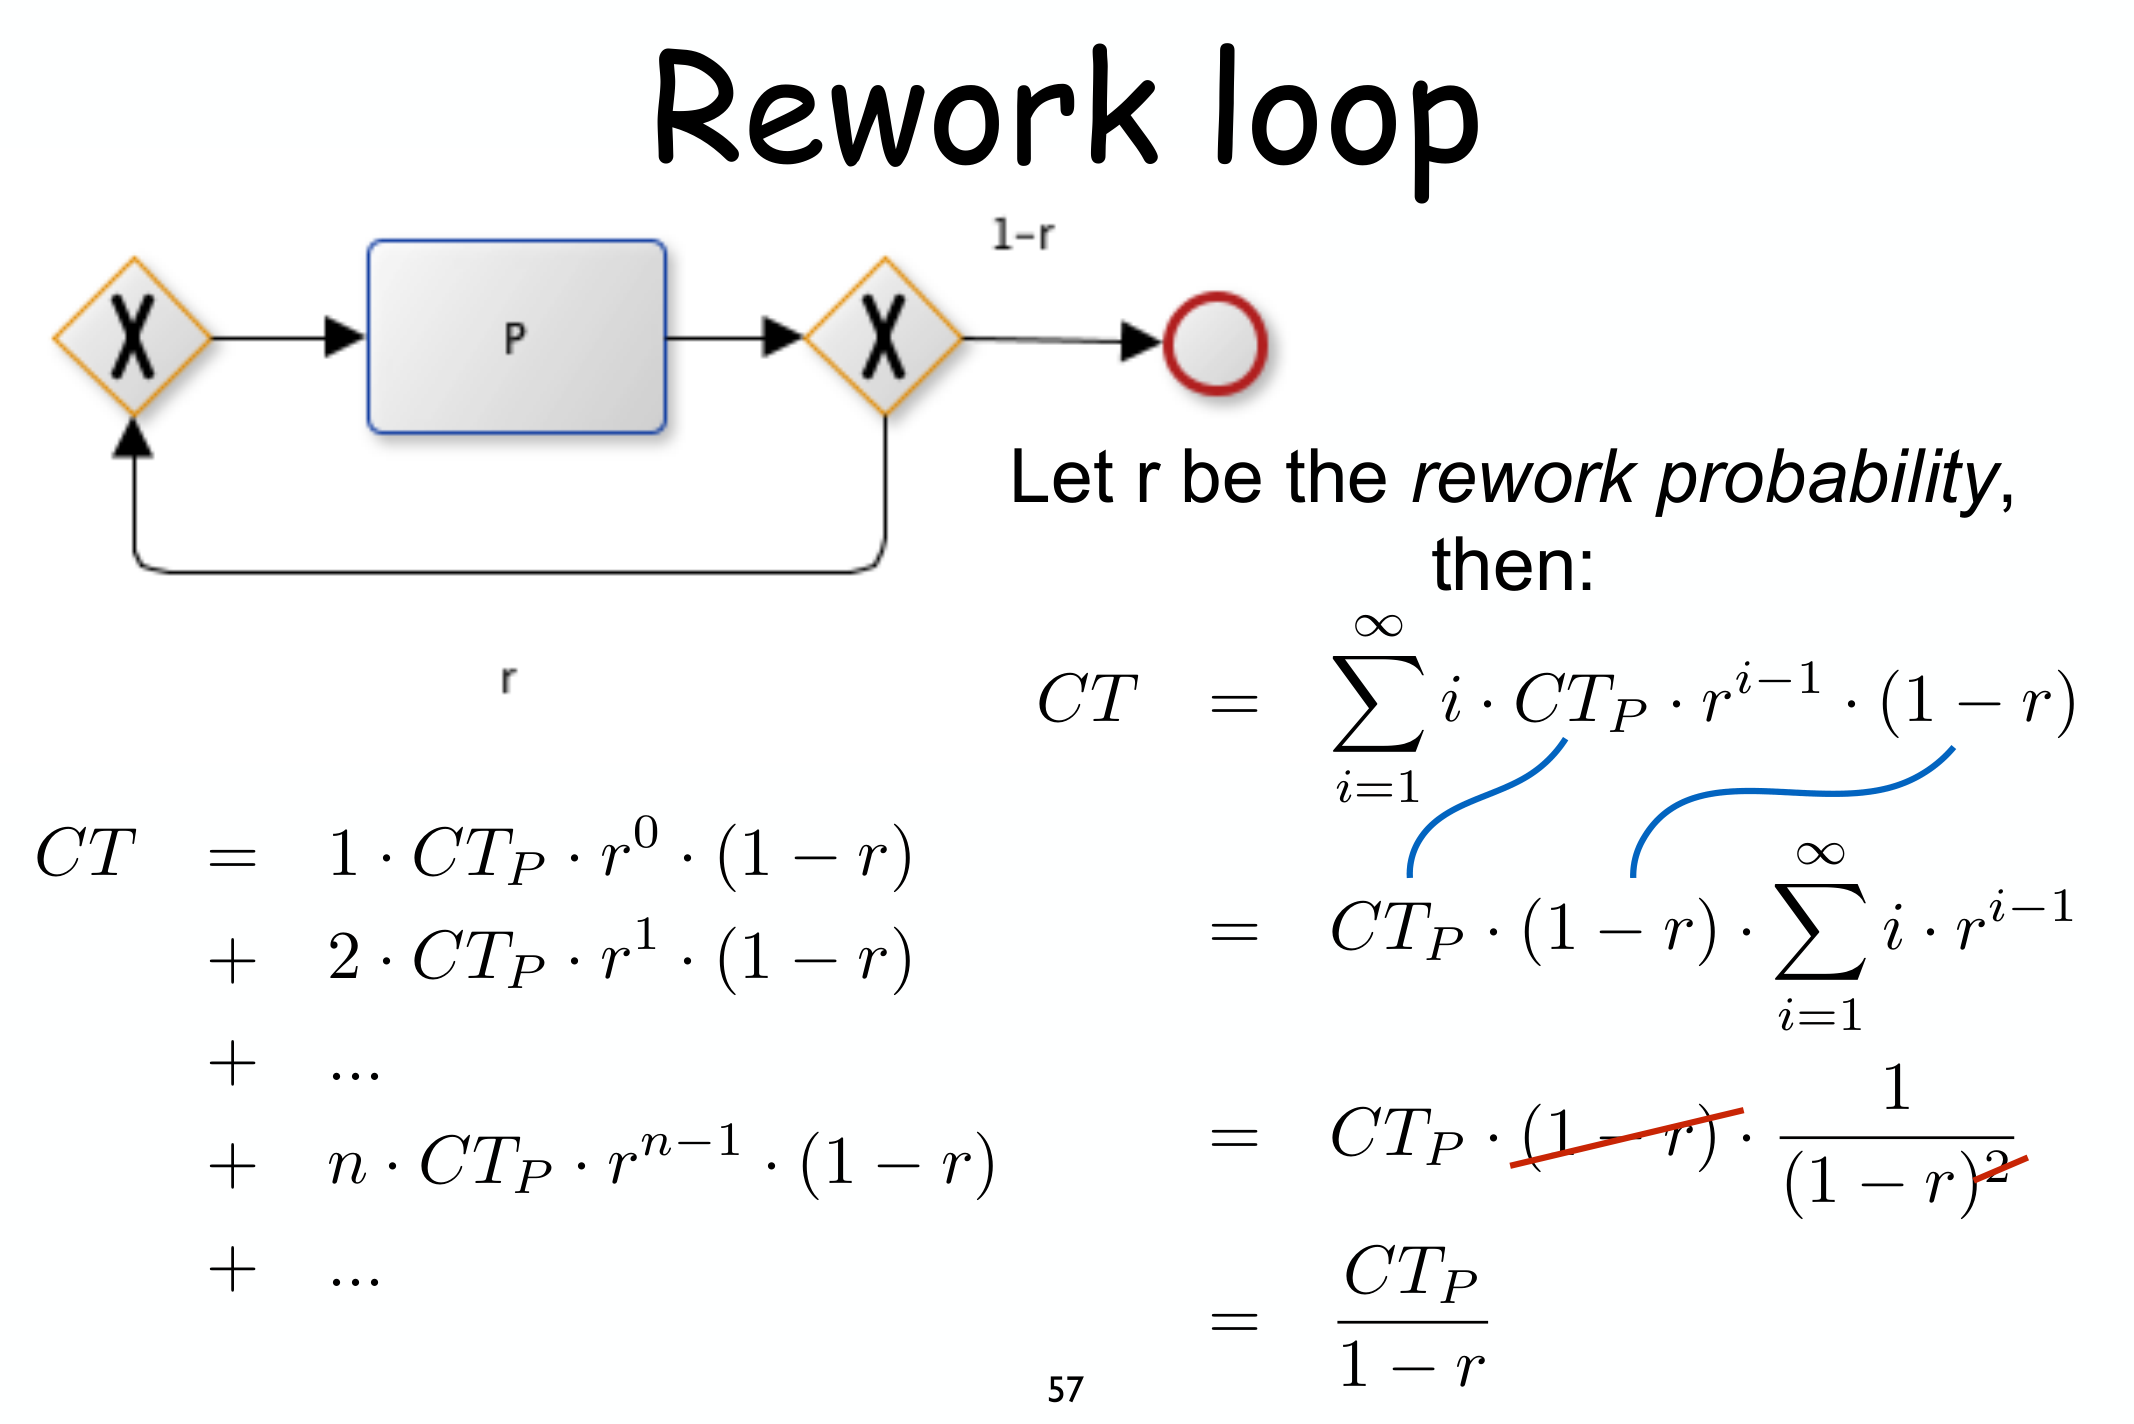
\includegraphics[width=0.74\linewidth,height=0.34\textheight,keepaspectratio]{images/20-quantitative_p57_rework-loop.png}
\caption{Derivazione di $CT = CT_P/(1-r)$: si somma $i \cdot CT_P \cdot r^{i-1}(1-r)$ su tutti i possibili numeri di ripetizioni $i$; la serie $\sum i\, r^{i-1}$ è quella nota dell'analisi (converge a $1/(1-r)^2$), e i due fattori $(1-r)$ si semplificano.}
\end{figure}

\begin{boxtheorem}{Rework loop (0 o più volte)}
Se invece $P$ può essere \textbf{saltato del tutto} (eseguito 0 volte con probabilità $1-r$, e così via): \(CT = \frac{r \cdot CT_P}{1-r}\)

\emph{Intuizione:} è esattamente il caso "1 o più volte" \textbf{meno} una singola esecuzione di $P$ già "scontata": \(\frac{CT_P}{1-r} - CT_P = \left(1-(1-r)\right)\cdot\frac{CT_P}{1-r} = \frac{r\cdot CT_P}{1-r}\)
\end{boxtheorem}

\section{\texorpdfstring{Oltre il cycle time: waiting vs processing, e Little's law}{Oltre il cycle time: waiting vs processing, e Little's law}}

Il cycle time da solo non dice \textbf{dove} si nasconde il tempo perso. Separarlo in waiting e processing chiarisce dove intervenire.

\begin{boxnote}{Waiting time vs processing time}
\begin{itemize}
\item \textbf{Waiting time}: la parte del cycle time in cui \textbf{nessuno lavora} sul caso (es. documenti in transito, attesa di un attore libero).
\item \textbf{Processing time}: il tempo in cui qualcuno \textbf{lavora davvero} sul caso.
\end{itemize}

In molti processi reali il waiting time è la parte \textbf{dominante} del cycle time (lavorazione a lotti, attori non disponibili, approvazioni che aspettano una firma).
\end{boxnote}

\begin{boxdefinition}{Theoretical cycle time e Cycle Time Efficiency}
Il \textbf{theoretical cycle time (TCT)} si calcola con le \textbf{stesse formule} del CT, ma usando i \textbf{processing time} al posto dei cycle time — è il tempo che il processo impiegherebbe se non ci fosse \textbf{mai} attesa.

La \textbf{Cycle Time Efficiency}: \(CTE = \frac{TCT}{CT}\)

\begin{itemize}
\item $CTE$ vicino a $1$: poco margine di miglioramento (a meno di cambiamenti radicali del processo).
\item $CTE$ vicino a $0$: \textbf{molto} margine, riducendo il waiting time.
\end{itemize}
\end{boxdefinition}

Un secondo strumento, indipendente dalla struttura del processo, lega il cycle time a due grandezze osservabili senza bisogno di conoscere i tempi delle singole attività.

\begin{boxdefinition}{Arrival rate e Work-In-Process}
\begin{itemize}
\item \textbf{Arrival rate} $\lambda$: numero medio di \textbf{nuovi casi} creati per unità di tempo.
\item \textbf{Work-In-Process (WIP)}: numero medio di casi \textbf{attivi} (non ancora completati) in un dato istante.
\end{itemize}
\end{boxdefinition}

\begin{boxtheorem}{Little's law}
In un sistema \textbf{stabile} (il numero di casi attivi non cresce all'infinito): \(WIP = \lambda \cdot CT\) equivalentemente: \(CT = \frac{WIP}{\lambda}\)

Formulata da John Little nel 1954 (dimostrata nel 1961), è universale: non serve sapere \textbf{nulla} della struttura interna del processo, bastano due grandezze \textbf{osservabili dall'esterno} (contare i casi attivi, contare gli arrivi).
\end{boxtheorem}

\begin{boxexample}{Uso pratico di Little's law}
Se in un anno (250 giorni lavorativi) arrivano 2500 domande, $\lambda = 10$/giorno. Campionando nel tempo si osservano in media $WIP=200$ domande attive contemporaneamente. Allora $CT = 200/10 = 20$ giorni — calcolato \textbf{senza mai} aver misurato il tempo di una singola domanda.
\end{boxexample}

\begin{boxtip}{La lettura operativa}
Dalla relazione $WIP = \lambda \cdot CT$: se $\lambda$ \textbf{aumenta} (più richieste in arrivo) e non si vuole far crescere il $WIP$ (cioè non si vuole più personale/spazio impegnato), l'\textbf{unica leva} è ridurre il $CT$ — lavorare più in fretta, snellendo il processo.
\end{boxtip}

\section{\texorpdfstring{Cost analysis}{Cost analysis}}

Le stesse idee della flow analysis si applicano al \textbf{costo} invece che al tempo: le formule per sequenza, XOR-block e rework restano \textbf{identiche}; cambia solo l'AND-block, dove — a differenza del tempo — i costi dei rami paralleli si \textbf{sommano} (il lavoro \emph{costa} comunque, anche se avviene in parallelo).

\begin{boxnote}{Cost = human resource cost + other cost}
\begin{itemize}
\item \textbf{Human resource cost}: costo orario della risorsa $\times$ processing time del task.
\item \textbf{Other cost}: costi fissi legati all'esecuzione del task, indipendenti dal tempo di lavoro umano (es. una fee fissa per un controllo esterno).
\end{itemize}
\end{boxnote}

\begin{figure}[!htb]
\centering
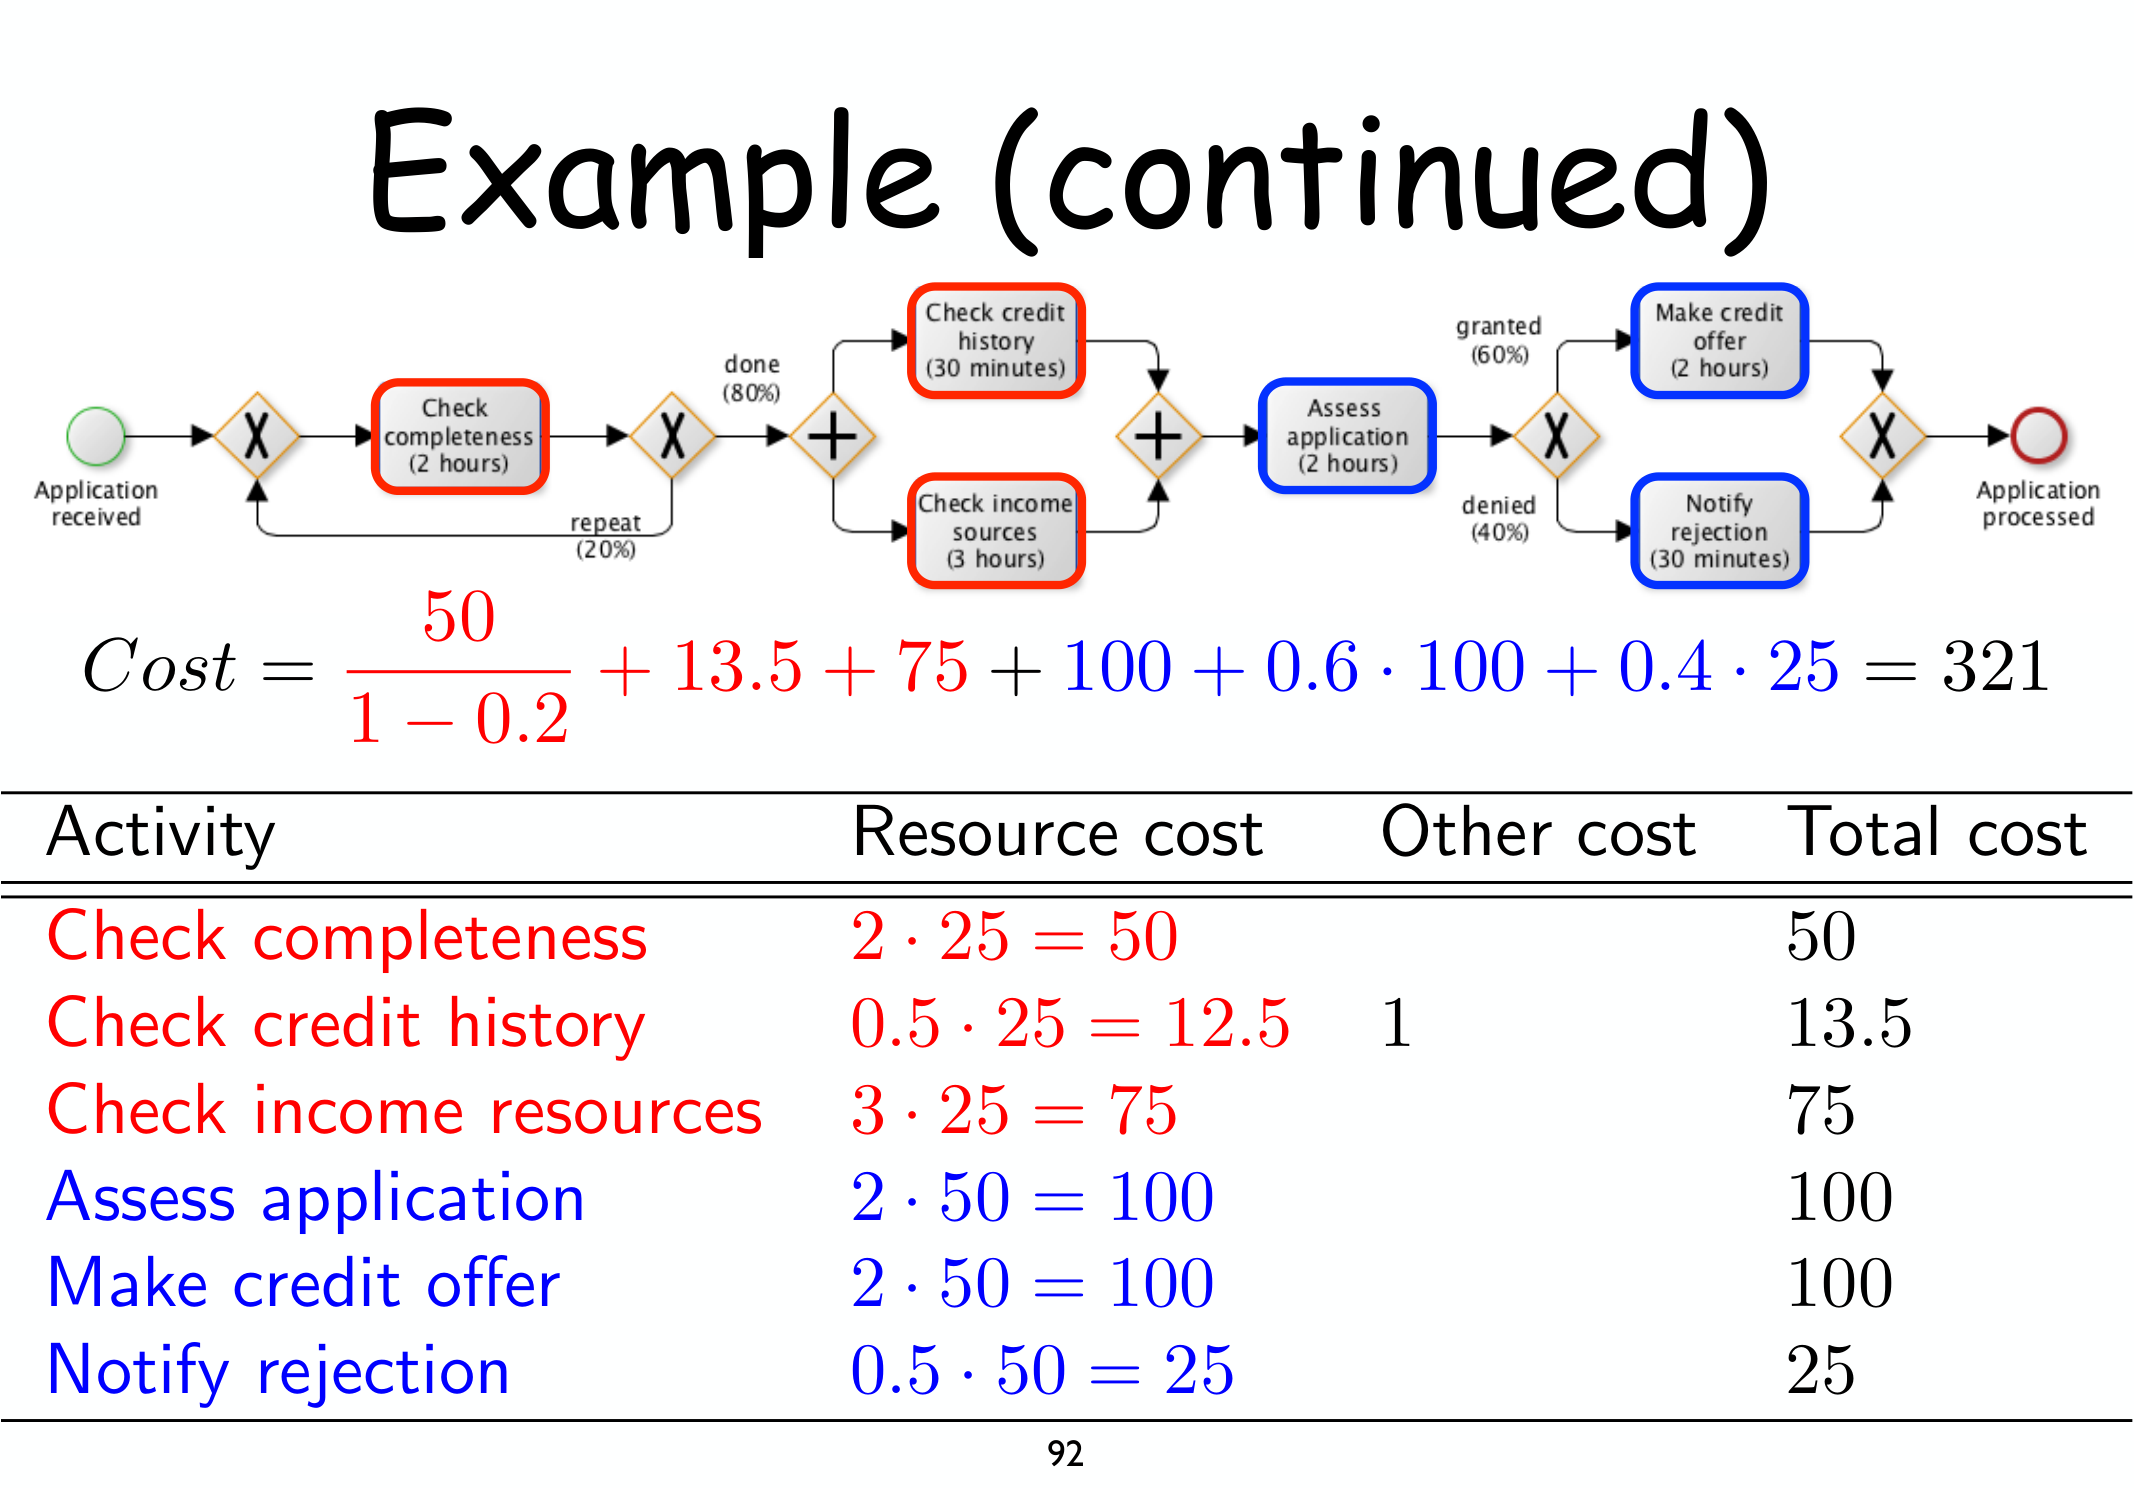
\includegraphics[width=0.74\linewidth,height=0.34\textheight,keepaspectratio]{images/20-quantitative_p92_cost-example.png}
\caption{Applicare le stesse regole di flow analysis al costo: il \textbf{rework} su "check completeness" (20\%) si tratta come nel cycle time ($/(1-0.2)$); i due rami paralleli "check credit history"/"check income sources" si \textbf{sommano} (non si prende il massimo, perché i costi si accumulano anche se il tempo no); lo XOR finale granted/denied si pesa con le rispettive probabilità (60\%/40\%). Costo medio totale: $\approx 321$€.}
\end{figure}

\section{\texorpdfstring{Limiti della flow analysis}{Limiti della flow analysis}}

La flow analysis è potente ma ha ipotesi forti, da tenere a mente prima di applicarla.

\begin{boxwarning}{Pitfall}
\begin{itemize}
\item Le formule valgono solo per processi \textbf{block-structured} (sequenza/XOR/AND/rework ben annidati): non si applicano a un grafo qualsiasi.
\item Servono \textbf{stime affidabili} dei tempi medi delle attività (da interviste o dai log) — l'intera analisi eredita l'incertezza di queste stime.
\item Non tiene conto del \textbf{carico}: quando il carico di lavoro sale e le risorse restano costanti, il waiting time \textbf{cresce} — un effetto che la flow analysis, basata su medie statiche, non cattura (servirebbero modelli di code).
\end{itemize}
\end{boxwarning}

\section{\texorpdfstring{Riepilogo}{Riepilogo}}

\begin{boxabstract}{Il quadro}
\begin{itemize}
\item Tre dimensioni di performance: \textbf{time}, \textbf{finance}, \textbf{quality} — misurate da KPI concreti.
\item \textbf{Flow analysis}: cycle time di sequenza (somma), XOR-block (media pesata), AND-block (massimo), rework loop ($CT_P/(1-r)$ o $r\cdot CT_P/(1-r)$).
\item \textbf{CTE} = TCT/CT misura quanto margine di miglioramento resta riducendo le attese.
\item \textbf{Little's law} ($WIP = \lambda \cdot CT$) collega arrival rate, work-in-process e cycle time \textbf{senza} bisogno della struttura interna del processo.
\item Le stesse regole (tranne l'AND-block, che diventa una somma) valgono per il \textbf{costo}.
\end{itemize}
\end{boxabstract}

Con la performance analysis chiudiamo la cassetta degli attrezzi \emph{quantitativa} del corso. Nell'ultima lezione torniamo ai workflow net per affrontare un problema pratico: cosa fare quando un processo \textbf{non} è sound — come \textbf{diagnosticarlo} e \textbf{ripararlo}. $\rightarrow$ \hyperref[ch:21]{21 — WFnets Diagnosis}